\chapter{Estratégias de Abordagem aos Problemas} \label{cap:abordagem}
Nesta secção vamos analisar os procedimentos, tecnologias e conceitos utilizados no desenvolvimento deste projeto.

\section{Modelo de Dados} \label{sec:dados}
Um dos componentes deste sistema é um repositório de dados, que irá conter as várias informações relacionadas com os clientes deste serviço. Na figura \ref{fig:relacoes} está representado de forma gráfica o modelo dos dados guardados neste repositório. \\

\begin{figure}[ht!]
\centering
\resizebox{120mm}{!}{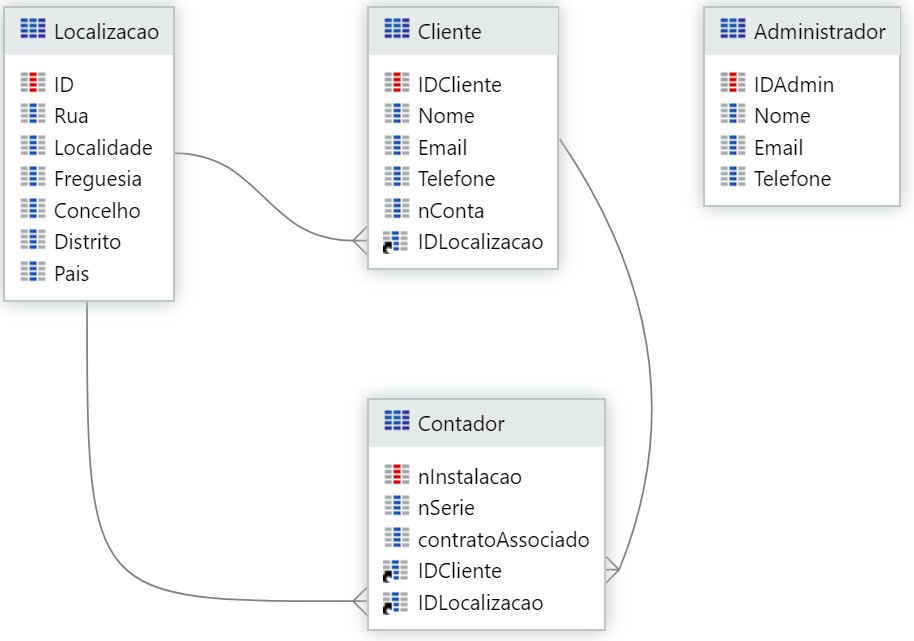
\includegraphics{diagramas/modeloDados.png}}
\caption{Arquitetura do sistema.}
\label{fig:relacoes}
\end{figure}

O elemento cliente representa um cliente do serviço que utiliza o sistema. Para cada cliente será registado um ID único (IDCliente), o seu nome, email, número de telefone/telemóvel e número de conta. \\
Também existem utilizadores com papel de administrador, para os quais registamos um ID único (IDAdmin), o seu nome, email e número de telefone/telemóvel. \\
Os clientes terão associado um ou mais contadores, pelo que para cada contador guardamos o seu número único de instalação, o seu número de série e o contrato e o cliente aos quais este contador está associado. \\
Cada contador tem uma localização, que representa o local onde o contador está instalado. Cada cliente tem também uma localização associada, que representa a sua morada principal para onde é, por exemplo, enviado o correio postal. Uma localização segue a estrutura normal de uma morada: rua, localidade, freguesia, concelho, distrito e país.

